\documentclass[a4paper,11pt]{article}


%%% fontenc
%\usepackage{fontspec,xunicode,xltxtra}
%\setmainfont{Times New Roman}
%\setsansfont{Source Sans Pro}
%\setmonofont{Source Sans Pro}

%%% xeCJK
\usepackage{xeCJK}
\setCJKmainfont[BoldFont=Adobe Heiti Std]{Adobe Song Std}
\setCJKsansfont[BoldFont=Adobe Heiti Std]{Adobe Song Std}
\setCJKmonofont[BoldFont=Adobe Heiti Std]{Adobe Song Std}
\XeTeXlinebreaklocale "zh"
\XeTeXlinebreakskip=0pt plus 1pt minus 0.1pt

\usepackage{xcolor}
\usepackage{graphicx}

%%% get total page number
\usepackage{lastpage}

%%% customized definition
\makeatletter
\def\sybtitle#1{\def\@sybtitle{#1}}
\def\sybauthor#1{\def\@sybauthor{#1}}
\def\sybdate#1{\def\@sybdate{#1}}
\sybtitle{}
\sybauthor{}
\sybdate{}
\def\sybmaketitle{
  \begin{center}
  \vspace*{.8in}
  {\huge\bfseries\@sybtitle}
  \par
  \vspace{.8in}
  {\Large\@sybauthor}
  \par
  \vspace{.2in}
  \@sybdate
  \vspace{.5in}
  \end{center}
}
\makeatother
\setlength{\parindent}{0pt}
\renewcommand{\today}{\number\month 月 \number\day 日, ~\number\year 年}
\def\lt{\textless}
\def\gt{\textgreater}
\renewcommand\contentsname{\bfseries 目~~录}
\newcommand\bs{\texttt{\symbol{'134}}} % input backslash sign
%\newcommand\bs{\string\} % same as above definition
\long\def\cmd#1{\par\vspace{.5em}\hspace*{2em}#1\vspace{.5em}\par}
\def\cstr#1{\texttt{\string#1}} % e.g. \cstr{\latex}
\long\def\runcode#1{\par\bigskip#1\bigskip\par}
% 我不想看到那么多的underful hbox,尤其是minted环境加上背景色之后
\hbadness=10000
% 适当放宽overful hbox的限制,运行2pt的溢出
\hfuzz=2pt
\parskip=3\lineskip


%%% change background color & add frame for enumerate enviroment
\usepackage{mdframed}
\newmdenv[backgroundcolor=blue!10,linewidth=0pt]{coloredframe}
\newenvironment{coloredenumerate}{
  \begin{coloredframe}
  \begin{enumerate}
}{
  \end{enumerate}
  \end{coloredframe}
}

%%% geometry
\usepackage[includehead,includefoot,hmargin=21mm,vmargin=10.5mm,
            headsep=12pt,headheight=25pt]{geometry}
%\usepackage[includehead,includefoot,hmargin=1.2in,vmargin=1in]{geometry}

%%% fancyhdr
\usepackage{fancyhdr}
\makeatletter
\fancypagestyle{main} {
  \fancyhf{} % clear header & footer
  \fancyhead[L]{\bfseries\@sybtitle}
  \fancyhead[R]{\thepage/\pageref*{LastPage}}
  \renewcommand{\headrulewidth}{0.4pt} % header line
  \renewcommand{\footrulewidth}{0pt} % footer line
}
\fancypagestyle{header} {
  \fancyhf{} % clear header & footer
  \fancyfoot[C]{\roman{page}}
  \renewcommand{\headrulewidth}{0pt} % header line
  \renewcommand{\footrulewidth}{0pt} % footer line
}
\makeatother

\usepackage{titlesec}
\titleformat{\part}{\centering\Large\bfseries}{第\,\thepart\,部分}{1em}{}
\titleformat{\section}{\large\bfseries}{\thesection}{1em}{}
\titleformat{\subsection}{\normalsize\bfseries}{\thesubsection}{1em}{}
%\titlespacing*{章节命令}{左边距}{上文距}{下文距}[右边距]
\titlespacing*{\section}{0pt}{2\baselineskip}{\parsep}


\usepackage{hyperref}

%%% perfect source code display
\usepackage{minted}
%\usemintedstyle{colorful}
\definecolor{srcbg}{rgb}{0.95,0.95,0.95}
\newminted{java}{linenos,tabsize=4,bgcolor=srcbg}
\newminted{xml}{linenos,tabsize=4,bgcolor=srcbg}
\newminted{cpp}{linenos,tabsize=4,bgcolor=srcbg}
\newminted{bash}{linenos,tabsize=4,bgcolor=srcbg}
\newminted{latex}{linenos,tabsize=4,bgcolor=srcbg}



\usepackage{xcolor}
\colorlet{HEADCOLOR}{red!50}
\colorlet{BRANCHCOLOR}{blue!50}
\colorlet{WORKCOLOR}{gray!50}
\colorlet{INDEXCOLOR}{cyan!50}
\colorlet{COMMITCOLOR}{green}

\usepackage{tikz}
\usetikzlibrary{shapes,arrows,positioning,calc,backgrounds,matrix,fit,decorations.pathreplacing}
\tikzset{
  basic-style/.style = {
    rectangle, rounded corners=2pt, draw, thick,
    fill=#1,
    minimum height=15pt,
    minimum width=1.5cm,
    inner sep=1pt
  },
  commit-style/.style = {
    basic-style=COMMITCOLOR
  },
  index-style/.style = {
    basic-style=INDEXCOLOR,
    minimum width=2.5cm
  },
  work-style/.style = {
    basic-style=WORKCOLOR,
    minimum width=2.5cm
  },
  branch-style/.style = {
    basic-style=BRANCHCOLOR
  },
  head-style/.style = {
    basic-style=HEADCOLOR
  },
  cmd-style/.style = {
    #1=5pt
  },
  cmd-style/.default = right,
  main-style/.style = {
    execute at end picture = {
      \begin{pgfonlayer}{background}
        \path[fill=gray!20,rounded corners]
          ([xshift=-0.2cm,yshift=-0.2cm]current bounding box.south west) rectangle
          ([xshift=0.2cm,yshift=0.2cm]current bounding box.north east);
          %(current bounding box.south west) rectangle
          %  (current bounding box.north east);
        \end{pgfonlayer}
    }
  },
  file-style/.style = {
    draw=red, fill=yellow!30, inner sep=2pt
  },
  dir-style/.style = {
    fill=green!50,inner sep=2pt
  },
  dir-bg-style/.style = {
    fill=cyan!30,rounded corners
  },
  every edge/.style = {draw, ->, >=latex', thick}
}

%%%%% new definitions %%%%%

\newlength\commitDistance
\setlength\commitDistance{0.5cm}
\newlength\indexWorkDistance
\setlength\indexWorkDistance{2\commitDistance}

\newcommand\displayName[1]{\ttfamily\bfseries #1}
\newcommand\commandName[1]{\ttfamily\bfseries\small #1}

\def\createNode style:#1 name:#2 display:#3 direct:#4 distance:#5 to:#6;{
  \node [#1, #4=#5 of #6] (#2) {#3}
        edge [#4] (#6);
}
\def\createCommit name:#1 display:#2 direct:#3 to:#4;{
  \node [commit-style, #3=\commitDistance of #4] (#1) {#2}
        edge [#3, COMMITCOLOR] (#4);
}
\def\createBranch name:#1 display:#2 direct:#3 to:#4;{
  \node [branch-style, #3=0.75\commitDistance of #4] (#1) {#2}
        edge [#3, BRANCHCOLOR] (#4);
}
\def\createHead direct:#1 to:#2;{
  \node [head-style, #1=0cm of #2] (head) {\displayName HEAD};
}
\def\createIndex to:#1;{
  \node [index-style, below=2\commitDistance of #1] (index) {\displayName Index};
}
\def\createWork to:#1;{
  \node [work-style, below=2\commitDistance of #1] (work) {\displayName Work DIR};
}

\newcommand\makeOutline{
  %\useasboundingbox (-0.1,-3.6) rectangle (10.7,2);
  \node[right] (dumy) at (0,0) {\dots};
  \createCommit name:a display:{\displayName A} direct:right to:dumy;
  \createCommit name:b display:{\displayName B} direct:right to:a;
  \createCommit name:c display:{\displayName C} direct:right to:b;
  \createCommit name:d display:{\displayName D} direct:right to:c;
  \createCommit name:e display:{\displayName E} direct:right to:d;

  \createIndex to:c;
  \createWork to:index;
}

\newcommand\createMatrix[2]{
  \matrix [
    matrix of nodes,
    nodes={rectangle,draw=red,fill=yellow!30,minimum width=1.3cm,font=\ttfamily\small,inner sep=2pt},
    row sep=-\pgflinewidth,
    column sep=-\pgflinewidth,
  ] (m#1) at #2 {
    \textcolor{blue}{list-#1}\\
    a.h\\
    b.h\\
    c.h\\
    $d_{v#1}.h$\\
  };
}

\newcommand\createHashMatrix[2]{
  \matrix [
    matrix of nodes,
    nodes={rectangle,draw=red,fill=yellow!30,minimum width=1.3cm,font=\ttfamily\small,inner sep=2pt},
    row sep=-\pgflinewidth,
    column sep=-\pgflinewidth,
  ] (m#1) at #2 {
    \textcolor{blue}{hash-#1}\\
    a47c3\\
    b325c\\
    c10b9\\
    \textcolor{cyan}{da98#1}\\
  };
}

\usepackage{calc} % for \real control sequence
%%%%%%%%%%%%%%%%%%%%%
\newlength {\boxw}
\newlength {\boxh}
\newlength {\boxd}
\newlength {\boxroundness}
\newlength {\boxshadowsize}
\newlength {\shadowiter}
\newlength {\innersep}


\setlength {\boxshadowsize}{6pt}
\setlength {\boxroundness}{3pt}

\newsavebox {\shadowblockbox}
\newenvironment{shadowblock}[4] % {minipage width}{fill color}{draw color}{inner sep}
{\def\fillcolor{#2}\def\drawcolor{#3}%
  \setlength {\innersep}{#4}%
  \begin{lrbox}{\shadowblockbox}\begin{minipage}{#1}}
{\end{minipage}\end{lrbox}
  % draw the textbox
  \settowidth {\boxw}{\usebox{\shadowblockbox}}   % get box's width
  \settoheight {\boxh}{\usebox{\shadowblockbox}}  % get box's height
  \settodepth {\boxd}{\usebox{\shadowblockbox}}   % get box's depth

  \addtolength {\boxh}{\boxd}
  \addtolength {\boxw}{2\boxroundness}
  \addtolength {\boxh}{2\boxroundness}
  \addtolength {\boxw}{2\innersep}
  \addtolength {\boxh}{2\innersep}

  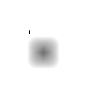
\begin{tikzpicture}
    % draw the shadow
    \foreach \x in {0,0.05,...,1} {
      \setlength{\shadowiter}{\boxshadowsize*\real{\x}}
      \fill[xshift=\boxshadowsize-1pt,yshift=-\boxshadowsize+1pt,
          black,opacity=0.04,rounded corners=\boxroundness]
          (\shadowiter,\shadowiter) rectangle +(\boxw-2\shadowiter,\boxh-2\shadowiter);
    }
    % draw the box border
    \filldraw[fill=\fillcolor,draw=\drawcolor,rounded corners=\boxroundness]
        (0,0) rectangle (\boxw,\boxh);
    % draw the content
    \node[xshift=\boxroundness,yshift=\boxroundness,inner sep=\innersep,outer sep=0pt,anchor=south west]
        at (0,0) {\usebox{\shadowblockbox}};
  \end{tikzpicture}
}

\newcommand\gitcmd[1]{%
%\begin{center}
%  \noindent\fcolorbox{white}{yellow!20}{%
%    \begin{minipage}{.7\textwidth}
%      \centering\Large
%      \texttt{#1}
%    \end{minipage}}
%\end{center}

\begin{center}
  \begin{shadowblock}{0.9\textwidth}{yellow!50}{black!50}{0pt}
  \centering\Large
  \texttt{#1}
  \end{shadowblock}
\end{center}
}

%\newsavebox{\framedtextbox}
%\newenvironment{framedtext}[1] % minipage width
%{\begin{lrbox}{\framedtextbox}\begin{minipage}{#1}\centering}
%{\end{minipage}\end{lrbox}
%  % put box in a tikz node, and draw the node.
%  \begin{tikzpicture}
%    \node [fill=gray!20,rounded corners] at (0,0) {\usebox{\framedtextbox}};
%  \end{tikzpicture}
%}
\newenvironment{framedtext}
{\begin{center}\begin{shadowblock}{0.7\textwidth}{gray!20}{red}{10pt}\ttfamily}
{\end{shadowblock}\end{center}}

\newcommand\surrounded[1]{
  \textless#1\textgreater
}

\newcommand\optionalSurrounded[1]{
  [\textless#1\textgreater]
}


\sybtitle{Algorithm Notes}
\sybauthor{孙延宾}
\sybdate{\today}

\begin{document}
  \tt % I love Typewriter font.
%%%%%%%% the title page and toc %%%%%%%%%%
  \pagestyle{header}
  \sybmaketitle
  \tableofcontents
  \newpage

%%%%%%% the main content %%%%%%%%%
  \pagestyle{main}
  \setcounter{page}{1}

  \section[rsync核心算法]{rsync核心算法}
  aaa

  \section[伙伴算法简易实现]{伙伴算法简易实现}
  \begin{center}
    % Requires \usepackage{graphicx}
    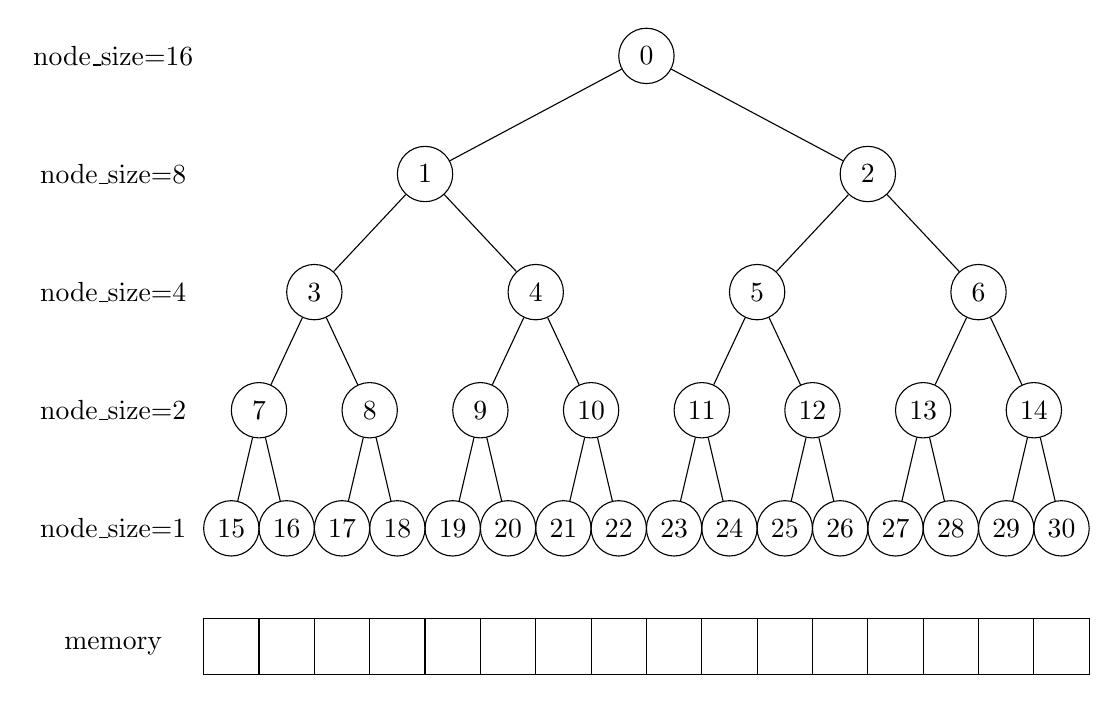
\begin{tikzpicture}
  [every node/.style={minimum size=20pt, inner sep=2pt},
   tree-node/.style={draw,circle},
   side-node/.style={},
   memo-node/.style={draw,rectangle},
   level 1/.style={sibling distance=160pt}, % 8 * 20pt
   level 2/.style={sibling distance=80pt}, % 4 * 20pt
   level 3/.style={sibling distance=40pt}, % 2 * 20pt
   level 4/.style={sibling distance=20pt}] % 1 * 20pt
  \node [tree-node] (root) {0}
    child {
      node [tree-node] {1}
        child {
          node [tree-node] {3}
            child {
              node [tree-node] {7}
                child {
                  node [tree-node] {15}
                    child [grow=down] {
                      node [memo-node] {} edge from parent[draw=none]
                        child [grow=left] {node [side-node] {memory} edge from parent[draw=none]}
                    }
                    child [grow=left] {
                      node [side-node] {node\_size=1} edge from parent[draw=none]
                        child [grow=up] {
                          node [side-node] {node\_size=2} edge from parent[draw=none]
                            child [grow=up] {
                              node [side-node] {node\_size=4} edge from parent[draw=none]
                                child [grow=up] {
                                  node [side-node] {node\_size=8} edge from parent[draw=none]
                                    child [grow=up] {
                                      node [side-node] {node\_size=16} edge from parent[draw=none]
                                    }
                                }
                            }
                        }
                    }
                }
                child {
                  node [tree-node] {16}
                    child [grow=down] {node [memo-node] {} edge from parent[draw=none]}
                }
            }
            child {
              node [tree-node] {8}
                child {
                  node [tree-node] {17}
                    child [grow=down] {node [memo-node] {} edge from parent[draw=none]}
                }
                child {
                  node [tree-node] {18}
                    child [grow=down] {node [memo-node] {} edge from parent[draw=none]}
                }
            }
        }
        child {
          node [tree-node] {4}
            child {
              node [tree-node] {9}
                child {
                  node [tree-node] {19}
                    child [grow=down] {node [memo-node] {} edge from parent[draw=none]}
                }
                child {
                  node [tree-node] {20}
                    child [grow=down] {node [memo-node] {} edge from parent[draw=none]}
                }
            }
            child {
              node [tree-node] {10}
                child {
                  node [tree-node] {21}
                    child [grow=down] {node [memo-node] {} edge from parent[draw=none]}
                }
                child {
                  node [tree-node] {22}
                    child [grow=down] {node [memo-node] {} edge from parent[draw=none]}
                }
            }
        }
    }
    child {
      node [tree-node] {2}
        child {
          node [tree-node] {5}
            child {
              node [tree-node] {11}
                child {
                  node [tree-node] {23}
                    child [grow=down] {node [memo-node] {} edge from parent[draw=none]}
                }
                child {
                  node [tree-node] {24}
                    child [grow=down] {node [memo-node] {} edge from parent[draw=none]}
                }
            }
            child {
              node [tree-node] {12}
                child {
                  node [tree-node] {25}
                    child [grow=down] {node [memo-node] {} edge from parent[draw=none]}
                }
                child {
                  node [tree-node] {26}
                    child [grow=down] {node [memo-node] {} edge from parent[draw=none]}
                }
            }
        }
        child {
          node [tree-node] {6}
            child {
              node [tree-node] {13}
                child {
                  node [tree-node] {27}
                    child [grow=down] {node [memo-node] {} edge from parent[draw=none]}
                }
                child {
                  node [tree-node] {28}
                    child [grow=down] {node [memo-node] {} edge from parent[draw=none]}
                }
            }
            child {
              node [tree-node] {14}
                child {
                  node [tree-node] {29}
                    child [grow=down] {node [memo-node] {} edge from parent[draw=none]}
                }
                child {
                  node [tree-node] {30}
                    child [grow=down] {node [memo-node] {} edge from parent[draw=none]}
                }
            }
        }
    };
\end{tikzpicture}
    %\caption{buddy system}\label{fig:buddy}
  \end{center}


  从伙伴算法看满二叉树的一些特性:
  \begin{description}
    \item[total\_leaf\_size] 满二叉树的叶子节点总数
    \item[level] 满二叉树的层级,范围0-max\_depth
    \item[node\_size] 每个level上节点的size
    \item[index] 某个节点在满二叉树数组中的索引
    \item[offset] 某一个节点对应的内存单元映射到叶子节点数组中的下标(offset)
  \end{description}
  total\_leaf\_size是已知的,即buddy system管理的内存单元总数。
  $$ max\_depth = \log_2total\_leaf\_size$$
  每个level上第一个左子树的index为$2^{level} - 1$
  \begin{align*}
    offset & = [index - (2^{level} - 1)] * node\_size \\
           & = (index + 1) * node\_size - 2^{level} * node\_size \\
           & = (index + 1) * node\_size - 2^{level} * 2^{max\_depth - level} \\
           & = (index + 1) * node\_size - 2^{max\_depth} \\
           & = (index + 1) * node\_size - total\_leaf\_size \\
  \end{align*}
  可见,无论哪个level,第一个左子树(最左边的节点)对应到叶子节点数组中的下标总是0.

  \section[字符串匹配的KMP算法]{字符串匹配的KMP算法}

  \section[字符串匹配的Boyer-Moore算法]{字符串匹配的Boyer-Moore算法}
  
  \section[寻找小于N的所有素数]{寻找小于N的所有素数}
  Sieve筛选算法用于寻找小于N的所有素数。\par
  \inputminted[linenos,tabsize=4,bgcolor=srcbg]{cpp}{srcdir/Sieve.c}
  
  筛选的方法是:\\
  首先去掉2的倍数,然后去掉3的倍数,然后去掉4的倍数,然后,...,
  直到去掉所有sqrt(n)的倍数,如下表:\par
  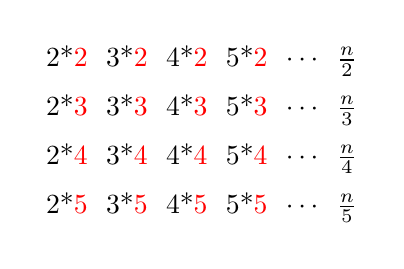
\begin{tikzpicture}
    \matrix [matrix of nodes]
    {
      2*\textcolor{red}{2} & 3*\textcolor{red}{2} & 4*\textcolor{red}{2} & 5*\textcolor{red}{2} & $\cdots$ & $\frac{n}{2}$ \\
      2*\textcolor{red}{3} & 3*\textcolor{red}{3} & 4*\textcolor{red}{3} & 5*\textcolor{red}{3} & $\cdots$ & $\frac{n}{3}$ \\
      2*\textcolor{red}{4} & 3*\textcolor{red}{4} & 4*\textcolor{red}{4} & 5*\textcolor{red}{4} & $\cdots$ & $\frac{n}{4}$ \\
      2*\textcolor{red}{5} & 3*\textcolor{red}{5} & 4*\textcolor{red}{5} & 5*\textcolor{red}{5} & $\cdots$ & $\frac{n}{5}$ \\
    };
  \end{tikzpicture}
  
  一般来说,任意一个小于sqrt(n)的数p,我们要去掉:\\
  2*p, 3*p, 4*p, 5*p, $\cdots$, p*p, (p+1)*p, (p+2)*p, $\cdots$\\
  观察一下可以发现,p*p以前的数字,在处理2、3、4、5、$\cdots$、(p-1)*p的倍数时
  都已经去掉了,所以对于p,我们从p*p开始移除。
  
  另外,为何只处理小于等于sqrt(n)的数字呢(上表中一直处理到n),从上面的说明可以知道,
  如果$p>sqrt(n)$,$p*p>n$,无需处理,而p*p之前的数字都已经移除了,
  也无需处理,所以如果$p>sqrt(n)$,则p无需处理。
  
  该方法的缺点是占用内存太大!

  \part[位操作算法实例]{位操作算法实例}
  aaa



\end{document}
